% !TEX TS-program = pdflatex
% !TEX encoding = UTF-8 Unicode

% This is a simple template for a LaTeX document using the "article" class.
% See "book", "report", "letter" for other types of document.

\documentclass[a4paper, 12pt]{article} % use larger type; default would be 10pt

\usepackage[utf8]{inputenc} % set input encoding (not needed with XeLaTeX)

%%% Examples of Article customizations
% These packages are optional, depending whether you want the features they provide.
% See the LaTeX Companion or other references for full information.

%%% PAGE DIMENSIONS
\usepackage{geometry} % to change the page dimensions
\geometry{a4paper} % or letterpaper (US) or a5paper or....
% \geometry{margin=2in} % for example, change the margins to 2 inches all round
% \geometry{landscape} % set up the page for landscape
%   read geometry.pdf for detailed page layout information

\usepackage{graphicx} % support the \includegraphics command and options
\usepackage{subfig}
\usepackage{amsmath}
\usepackage{tabularx}
% \usepackage[parfill]{parskip} % Activate to begin paragraphs with an empty line rather than an indent

%%% PACKAGES
\usepackage{booktabs} % for much better looking tables
\usepackage{array} % for better arrays (eg matrices) in maths
\usepackage{paralist} % very flexible & customisable lists (eg. enumerate/itemize, etc.)
\usepackage{verbatim} % adds environment for commenting out blocks of text & for better verbatim
\usepackage{subfig} % make it possible to include more than one captioned figure/table in a single float
% These packages are all incorporated in the memoir class to one degree or another...
\usepackage{fontspec}
\usepackage{pdflscape}
\usepackage{xcolor}
\usepackage{multirow}
\newcolumntype{C}[1]{>{\centering\let\newline\\\arraybackslash\hspace{0pt}}m{#1}}
\usepackage{tikz}
\newcommand*\circled[1]{\tikz[baseline=(char.base)]{
            \node[shape=circle,draw,inner sep=2pt] (char) {#1};}}
%%% HEADERS & FOOTERS
\usepackage{fancyhdr} % This should be set AFTER setting up the page geometry
\pagestyle{fancy} % options: empty , plain , fancy
\renewcommand{\headrulewidth}{0pt} % customise the layout...
\lhead{}\chead{}\rhead{}
\lfoot{}\cfoot{\thepage}\rfoot{}

%%% SECTION TITLE APPEARANCE
\usepackage{sectsty}
\allsectionsfont{\sffamily\mdseries\upshape} % (See the fntguide.pdf for font help)
% (This matches ConTeXt defaults)
\setmainfont{Times New Roman}
%%% ToC (table of contents) APPEARANCE
\usepackage[nottoc,notlof,notlot]{tocbibind} % Put the bibliography in the ToC
\usepackage[titles,subfigure]{tocloft} % Alter the style of the Table of Contents
\usepackage{csquotes}
\usepackage{natbib}
\usepackage{hyperref}
\usepackage{longtable}
\usepackage{rotating}
\setcitestyle{round}
\renewcommand{\cftsecfont}{\rmfamily\mdseries\upshape}
\renewcommand{\cftsecpagefont}{\rmfamily\mdseries\upshape} % No bold!
\newcommand{\var}[1][\textit]{#1}

%%% END Article customizations

%%% The "real" document content comes below...

\title{\textbf{Automated Valuation Model: An Application in Japanese Rental Markets}}

\author{Lewen Guo\thanks{Independent Researcher} \  Yuichiro Kawaguchi\thanks{Graduate School of Business and Finance, Waseda University} \  William Cheung\thanks{Graduate School of Business and Finance, Waseda University}}

%\date{} % Activate to display a given date or no date (if empty),
         % otherwise the current date is printed 

\begin{document}

\maketitle
\begin{abstract}
Researchers in real estate and practitioners in mass appraisal industry have developed Automated Valuation Models (AVMs) for estimating housing prices in different housing markets. However, few of them develop AVMs in rental market. By constructing a unique micro-level housing rental dataset, we build two residential rental AVMs for five districts in Tokyo using two different methods -OLS and Ordinary Kriging- in this study. The accuracy metrics from our training and test sets illustrate ambiguous preferences of which method performs better in terms of R-square and RMSE. Besides, we investigate the roles of spatial variables based on our baseline hedonic regression models. Spatial variables -latitudes, longitudes and distances to Tokyo Station- are crucial in determining the housing rents in Tokyo residential market. In addition, we conduct Kriging Error Decomposition analysis based on relative likelihood ratios and find that Ordinary Kriging method, despite its simplicity in interpolation of spatial data, may lead to information losses in modeling the rental functions as the method omits important housing attributes.
\end{abstract}
\medskip
\textbf{JEL classification:} R3, R32.

\noindent \textbf{Keywords:} Automated Valuation Model, Hedonic Pricing Model, Kriging, Spatial Pricing
\section{Introduction}

As technology advances, the Automated Valuation Model (shorted as AVM hereinafter) is attracting increasingly attention among researchers in real estate and practitioners in mass appraisal industry. We quote the definition from International Association of Assessing Officers (shorted as IAAO hereinafter) for AVM:

\blockquote{\textit{An automated valuation model (AVM) is a mathematically based computer software program that produces an estimate of market value based on market analysis of location, market conditions, and real estate characteristics from information that was previously and separately collected. The distinguishing feature of an AVM is that it is an estimate of market value produced through mathematical modeling. Credibility of an AVM is dependent on the data used and the skills of the modeler producing the AVM.}}

The origin of the AVM research may date back to late 1980s where most of the researchers and practitioners use traditional models such as cost approach, income approach, comparable sales method as well as income approach as theoretic basis to build their AVMs or to conduct mass appraisal analysis. During that period, the multiple regression analysis (MRA) or the hedonic regression technics are widely used in their research\citep{uspap, d1986goodness}. After IAAO set a standard for AVM in the industry in 2003, the AVM is officially distinguished from traditional appraisal method in which an appraiser physically inspects properties and relies more on experience and judgement to analyze the data and develop an estimate of market value. Not until 1990s with the availability of various statistics packages, have a substantial number of empirical works in related to mass appraisals and predictions of housing price been conducted. It is from then, in our understanding, AVM is being recognized as an important independent research field in real estate economics and appraisal society. 

Existing literatures in this new field are heavily centered in building house-price-related AVMs \citep{faishal2005automated, garcia2008ann+}, while existing literature has seldom endeavored to construct rental AVM despite few have investigated and compared different methodologies which have been utilized on modeling the functions of housing rent \citep{brunauer2010additive, djurdjevic2008estimation, lochl2010modelling, seya2011empirical}. The reasons, from our perspectives, which lead to the blank in this rent-related field may lie in the following facts. First, it is difficult to collect rental data since such information is often exclusively owned by big-brand housing brokerages. Without high-quality data to analyze, there’s little space for researchers to conduct empirical studies. Second, the fact that no consensus has ever been reached in academia of how to construct a standardized model for modeling housing rents makes benchmarking a related study difficult which in turn disperses research interests among researchers.  

Despite this blank in rental market research, there’s an urgent need from the public that real estate market should be more transparent since real estate markets exhibit strong evidence that information asymmetry results in biased behaviors among market participants \citep{garmaise2003confronting}. Therefore, one of our objectives in this study is to alleviate information asymmetry by constructing an AVM where the rental of any room in our study areas could be estimated based on our models. Market participants and the general public can refer to AVM-based information before they make decisions. 

We select Japan as our study area because of the stability of rental prices after bubble burst \citep{shimizu}, which provides a temporal-controlled environment for testing cross-sectional data.\footnote{In this study, we can only obtain the cross-sectional data due to limitations in data-collecting process.} Japan is a stable developed country which suffered from housing bubbles and bubble burst. However, its housing rents remain almost unchanged after 2008, it is estimated the average of appreciation rate in Tokyo is only 0.7\% between 2008 and 2013 \citep{Statics}. The asking rents, in Japan, could also be interpreted as a proxy for the real transactional rents as landlords seldom altered their rents after posting the ads on brokerages \citep{seya2011empirical}. 

Practically, we construct a micro-level dataset which includes both micro-level attributes of individual houses and geographical coordinates resembling famous Boston Housing Price dataset \citep{harrison1978hedonic}. Our dataset is unique and abundant in terms of the attributes of houses and geographic representativeness, which could be extended to a panel dataset if necessary. 

We investigate the roles of spatial variables in Japanese rental markets. It is found that latitudes and longitudes in our sample areas are extremely crucial in determining the housing rents. The distance to Tokyo Station can explain part of variations in housing rents but cannot capture the spatial effects completely in our hedonic pricing models. Other structure variables exhibit similar characteristics as many hedonic pricing literatures summarized by \citet{sirmans2005composition}. We also build AVM based on both OLS and Ordinary Kriging Method, an interpolation method in geostatistics, which only takes geographic coordinates as inputs while could be used to estimate unknown rents. Our AVMs exhibit spatial heterogeneity across different regions in both OLS-based AVM and Kriging-based AVM.

We also compare the accuracy metrics of two different approaches -hedonic regression models (OLS) and Ordinary Kriging- in modeling AVM. The results indicate OLS performs better than Ordinary Kriging in 4 districts out of 5 in our sample. The failure to model rental function in Minato district warns us that simple methodology should be used with caution when constructing AVM. And splitting whole sample into training set and test set is almost mandatory to obtain appropriate interpretation.

This study has the following contributions. First, to our best knowledge, we are among the first to develop the AVM in rental market and the first few to investigate the roles of space in Japanese rental market. This fills the gap between the Japanese AVM research field and the leading AVM research in the world. Second, the AVMs that we have develop provide an important database for researchers and practitioners including appraisers, bankers, portfolio managers, government as well as the public. Third but not least, it is often cited in many papers \citep{cocco2000hedging} that real estate market is incomplete, and information is not as fully transparent as stock market. By providing an open-source AVM to the public, we can to some extend alleviate the Information Asymmetry in real estate market which will lead to a more efficient market in future. In addition, our research is useful to provide more precise estimated imputed rents for owner-occupied dwellings in the Japanese System of National Accounts.

The rest of the thesis is arranged as follows. Section 2 reviews existing literatures which use different methodologies to model housing price (rent) functions. Section 3 introduces data constructions and estimation methods. Section 4 shows the results and discussions. Section 5 concludes our findings and contributions. 

\section{Literature Review}
label{sec2}
In terms of methodologies that researchers use to develop AVMs, existing papers can be divided into roughly three mainstreams—regression-based methods, AI-based methods \citep{zurada2011comparison} and geostatistic-based methods. Regression-based methods can be further split into traditional assessment based on multiple regression analysis (MRA) methods or hedonic methods \citep{adair1988application, mark1988multiple, do1992neural, garrod1992valuing, faishal2005automated}, spatial regression methods in consideration of spatial autocorrelation \citep{anselin1990some, kelejian1998suggested} and spatial heterogeneity \citep{fotheringham2003geographically, fotheringham2015geographical}, and semiparametric model \citep{robinson1988root, anglin1996semiparametric, clapp2002predicting, fan2018local} and non-parametric model \citep{mcmillen2010estimation}. AI-based methods including famous Neural-Network(NN) based methods \citep{do1992neural, tay1992artificial, worzala1995exploration, mccluskey1996mass, borst1997evaluation, rossini1999accuracy, limsombunchai2004house, garcia2008ann+, peterson2009neural, mccluskey2012potential}, and Fuzzy Logic \citep{bagnoli1998theory, aurelio2006mass,guan2008adaptive} are becoming hotspots in the past two decades. And the popularity raised from keywords like ‘Big Data’, ‘Machine Learning’ among mass media and public makes such research field a cross-discipline of computer science and real estate economics. In contrast with AI-Method, Geostatistics, a branch of statistics which is widely used in spatial datasets, developed by South Africa engineering \citet{krige1951statistical} and is used for predict probability distributions of ore grades for mining operations. However, it is not until recently, geostatistics-based method is applied in real estate research \citep{kuntz2014geostatistical}.  

Despite intensive research available with different approaches especially in model specifications, no widely-accepted consensus had ever been reached in academia in terms of how to construct AVM. \citet{crone1992estimating} did an overall comparison of five regression models: three parametric and two non-parametric methods. They argue that parametric methods can yield higher accuracy, mean absolute error in this case, than non-parametric methods. In contrast, \citet{brunauer2010additive} drew an opposite conclusion in their paper that additive mixed regression models (AMM), non-parametric methods, are shown superior results in contrast to parametric method. The inconsistency of which method performs better appears in the works of AI-based method as well. \citet{mccluskey2012potential} summarize predictive performance of several works where comparisons between NN methods and hedonic regression are made. However, they find that there is no clear explanations and evidence of why, in most of time, NN methods would have better predictive performances. In early work of \citet{worzala1995exploration}, they argue the results of NN methods will vary depending on packages of software and the long run times of the same package.

The pros and cons of different methods are summarized as following: Hedonic price model and MRA model is easy to estimate, and coefficients are easy to interpret. But naïve OLS model cannot deal with non-linearity and all spatial problems. Spatial econometrics developed by \citet{anselin1990some} and \citet{kelejian1998suggested} can deal with spatial autocorrelation by adding a pre-specified spatial matrix into the regression equations. Empirical works suggest that, if setting spatial weights correctly, predicting power could increase if compared with non-spatial regressions. However, as \citet{martinetti2017approximate} argue in their paper, few literatures focus on how to address issues such as spatial heterogeneity, spatial autocorrelation, non-linearity and time invariance simultaneously. Geostatistics, which requires only geographical coordinates, is an easy-to-implement interpolation method. However, the kriging process, which excludes other possible explanatory variables may suffer information loss compared with regression methods and AI methods. 

Non-linearity methodologies such as local polynomial regression or additive hedonic regression can allow researchers to evaluate data without assuming the functional form in advance between dependent variables and independent variables. By modelling non-parametrically through P-splines, non-linearity and time-invariant effects could be partially wiped out \citep{brunauer2010additive}. But many of theoretic properties are difficult to understand and the computation requires a larger time as covariates increase \citep{opsomer1997fitting}.

Up to now, most of research focus on real estate housing price, few have investigated to construct AVM in rentals given the fact that rental markets are attached equal importance. Existing literatures which set predictive variable as rental or rental related data include the following: \citet{djurdjevic2008estimation} test hedonic model in Swiss market and find that their multilevel model has better predictive performance than segmented OLS models. \citet{lochl2010modelling} compared 4 models by using Swiss asking rental data from a publicly available web site. They find that GWR model which intends to solve the spatial heterogeneity, though not perfectly and still suffered from spatial autocorrelation, can provide better predictive accuracy than OLS and SAR models. \citet{seya2011empirical} are the first to investigate empirical comparisons among spatial econometrics, spatial statistics (kriging) and semiparametric models. Their works provide us an intuition of how suitable Japanese data are for testing rental functions. Vienna paper, however, focuses on more on dealing with non-linearity and models time-trend through P-splines non-parametrically \citep{brunauer2010additive}. These literatures provide us some sorts of benchmark to conduct empirical research. However, as far as we are concerned, no existing literature so far has modeled the housing rents by geostatistics, therefore our study is quite experimental and may require a number of tests and trials to obtain optimal results.  

\section{Data and Methodology}
\subsection{Dataset Construction}
We construct a unique dataset for analysis from two different sources. One dataset that we use throughout this thesis is “asking-rent” dataset constructed from one of the largest Japanese real estate brokerage company- “Athome”. This dataset is composed of asking rents for residential houses whose owners put their ads on Websites through “Athome”, and micro-level housing attributes of the underlying houses for rent. 

Since our interests are focused on constructing AVM for rental markets, which, from our perspectives, involves empirical analysis based on geographical data, we therefore obtain an additional “point” dataset to complement “asking-rent” dataset by adding the geographical coordinates of each house – latitudes and longitudes - into each single piece of data. The “point” dataset provided by Zenrin Corporation can fulfill our tasks in that this dataset collects geographical coordinates of all the residential buildings in a specified area, say, the whole residential houses in one specific district. The “point” dataset is updated until July 2017 and therefore it is suitable for our analysis. 

We merge the “point” dataset with “asking-rent” dataset in the following way: First, for each piece of data in “asking-rent” dataset, we query the address from “point” dataset to match the address of “asking-rent” dataset.\footnote{Since the address in “asking-rent” dataset is incomplete, we can only match the address of two datasets in block level. We then obtain a subsample of “point” dataset in the same block.   } Second, within a subsample of the same block, we match the floor number of the buildings in two datasets. Third, within the same block and the underlying building with the same floor number, we use the python package “fuzzywuzzy” to match the names of the buildings in two datasets.\footnote{The package “fuzzywuzzy” is a string matching toolbox in python using Levenshtein Distance to calculate the differences between sequences. It can output a ratio indicating similarity between two strings. A quick example is, if we put two sentences "fuzzy wuzzy was a bear", "wuzzy fuzzy was a bear" into the fuzz.ratio function of “fuzzywuzzy” package, the output ratio is 91. The code for matching the name of the buildings is available upon request.} We get “one-to-one” matching results and select the matched data whose fuzzy ratio is larger than 80. After data cleaning process, the final dataset resembles famous Boston Housing Price dataset \citep{harrison1978hedonic} where both micro-level of housing attributes and geographical coordinates are available for analysis.

For the purposes of data visualization, we obtain the mapping data and GIS-related data from Geospatial Information Authority of Japan. The mapping data includes base-map, road-map, and topographic map of district-level in Japan. Figure 1 shows the geographic plot of our final sample data.

\bigskip
 \centerline{\bf [\hyperref[fig1]{Figure 1}]}
\bigskip

\subsection{Variables Description}
\label{sec32}
We obtain 10892 pieces of data from the period of Jan 2018 to March 2018 within five districts in Tokyo.\footnote{In this study, we test the data of five districts in Tokyo which are Shinjuku, Minato, Sumida, Koutou, Setagaya. Our final dataset is cross-sectional since we delete the duplicated observations. Within our collection period, the values of the attributes and the rent for each underlying house are consistent in our data-cleaning process and there are no two different values for the same attributes of each underlying house.} We have 24 variables for each piece of data in our final dataset. The dependent variables are, \var{Unitrent} and \var{Logunitrent} representing rent per square meter and logarithm of rent per square meter, respectively. The numerical attributes for each piece of data are named and defined as the following: latitude and longitude of the house, \var{Latitude} and \var{Longitude}; floor area of the house for rent, \var{Floorarea}; number of rooms, \var{Room}; number of living rooms, \var{Living}; number of kitchens, \var{Kitchen}; number of storage room, \var{Storage}; number of dinner room, \var{Dinner}, management fee, \var{ManagementFee}; deposit fee, \var{Shikikin}; gratuity fee, \var{Reikin}; security money, \var{Hosyoukin}; floor number of the house, \var{Floornum}; total floor of the building where the underlying house lies in, \var{Totalfloor}; distance in kilometers to Tokyo Station, \var{DistToTokyo}; the time (in minutes) to walk to nearest station, \var{Accessibility}; the age of the building, \var{Age}; and the floor number of the house relative to the total floor of the underlying building, \var{RelativeFloor}. Dummy variables in our dataset are \var{DummyPark}, \var{DummyBikepark} and \var{DummyMaterial}, indicating whether the house has a car-parking lot, bike-parking lot and material used for construction is concrete.\footnote{The materials used for construction are roughly divided into two types – concrete and wood- in Japan. According to Statistics Japan Residential House and Land survey conducted in 2013, among 52.1 million houses in Japan 21.99 million (42.2\%) are concrete-made houses, while this number for wooden houses is 30.11 million (57.8\%).} We also construct district dummy variables for each district and in total we have five dummy variables: \var{DummyShinjuku}, \var{DummyKoutou}, \var{DummyMinato}, \var{DummySumida}, and \var{DummySetagaya}. We also include one categorical variable in our dataset. \var{Orientation} is a variable indicating the positioning of a house in relation to seasonal variations in the sun's path. In our dataset, there are eight different directions which indicate the different positioning of a house. Based on previous survey literatures \citep{green2003primer, sirmans2005composition}, we use the following terminologies to describe different types of variables:

\begin{itemize}
\item (Dummy) Structural Variables: \var{Floorarea}, \var{Room}, \var{Living}, \var{Kitchen}, \var{Storage}, \var{Dinner}, \var{ManagementFee}, \var{Shikikin}, \var{Reikin}, \var{Hosyoukin}, \var{Floornum}, \var{TotalFloor}, \var{RelativeFloor}, \var{Accessibility}, \var{Age}, \var{DummyPark}, \var{DummyBikepark} and \var{DummyMaterial}. 
\item Spatial Variables: \var{Latitude}, \var{Longitude} and \var{DistToTokyo}. 
\item District Dummy Variables: \var{DummyShinjuku}, \var{DummyKoutou}, \var{DummyMinato}, \var{DummySumida}, and \var{DummySetagaya}. 
\end{itemize}

\subsection{TrainTest Splitting and Hypothetical Dataset}
\label{sec33}
We separate the full dataset into training set and test set. By using the functions from scikit-learn, we split the full dataset randomly based on an 80\% to 20\% split ratio.\footnote{Scikit-learn is a python package for machine-learning. The function used to split train test data is sklearn.model\_selection.train\_test\_split.} The small-size sample data – approximately 10000 pieces in total – makes us determine 80\% to 20\% split ratio as our benchmark which enables us to obtain enough observations to perform accuracy test on test set.

For the purposes of predicting the rental price for all the properties within a specific area based on regression models, it is required that the attributes of unknown properties as the inputs of our AVM. However, actual house-specific data cannot be obtained since “point” dataset only has the building-level attributes but not house-level attributes. We, therefore, construct a hypothetical dataset based on “asking-rent” dataset and “point” dataset. For each piece of data in “point” dataset, we average the attributes of ten nearest-neighbors from “asking-rent” dataset based on their great circle distances and assign the mean value of these attributes, except for latitude and longitude, as the hypothetical values for the attributes of each single piece of data. We must admit here that these hypothetical data are only used for calculation of regression-based AVM since they are smoothed hypothetical data which cannot represent the true values.

\subsection{Model Specifications and Methodologies}
\subsubsection{Hedonic Pricing Model}
The origin of hedonic model can be traced back to late 1930s when \citet{court1939} first developed a hedonic pricing index for the automobile industry. However, it was not until late 1960s and early 1970s after \citet{lancaster1966new} developed a utility-generating microeconomic theory and \citet{rosen1974hedonic} constructed an equilibrium hedonic pricing model based on buyer and seller choices that researchers started to conduct empirical studies for estimating the functions of housing price. The Hedonic Pricing Model views the value of a house is contributed by the satisfaction that users gain from each separate attribute of the house. Due to its straightforward interpretation and simplicity in calculation, the Hedonic Pricing Model attracts attention from people in real estate appraisal as well. However, in real estate appraisal, the terminology used for Hedonic Regression Model is “Multiple Regression Analysis” though the statistics tool -OLS- that both economists and appraisers is the same. Despite inconsistency between two different research areas, the basic regression equation is summarized by \citet{sirmans2005composition} and generally takes the following form:

\bigskip
\centerline{ $Price=F(Physical Characteristics, Other Factors)$ }
\bigskip

\noindent Where the Physical Characteristics are typically, the physical attributes of a house, and Other Factors are the external factors which may, affect the housing price such as level of income within the area, GDP per capita, crime rate and so forth. 

Following previous hedonic rental literature \citep{djurdjevic2008estimation, lochl2010modelling, seya2011empirical}, we construct the hedonic regression model as our baseline regression and could be written as follows:
\begin{equation}
\label{eq1}
ln P = \alpha + \beta X + \epsilon
\end{equation}

\noindent Where $ln P$ is the logarithm of a vector of asking rents (N$\times$1, where N is the number of observations), $\alpha$ is the constant,  $\beta$ is a vector of coefficients (N$\times$1) and $X$ is a matrix of house attributes (N$\times$K, where K is the number of attributes). In our baseline hedonic regression models, we regress logarthmns asking rent per square meter, \var{Logunitrent} on both structural variables, and spatial variables. Structural variables are \var{Floorarea}, \var{Room}, \var{Living}, \var{Kitchen}, \var{Storage}, \var{Dinner}, \var{ManagementFee}, \var{Shikikin}, \var{Reikin}, \var{Hosyoukin}, \var{TotalFloor}, \var{Accessibility}, \var{Age}, \var{RelativeFloor}, \var{DummyPark}, \var{DummyBikepark}, and \var{DummyMaterial}, representing the structural characteristics of each house. Spatial variables are \var{Latitude}, \var{Longitude}, capturing the geographical location of each house. In addition to the baseline regression, we also include the \var{DistToTokyo} and district dummy variables in our regression to test what kind of roles can spatial variables play in determining the rental prices.

\subsubsection{Ordinary Kriging}
Ordinary kriging is used to estimate the unknown true values of points where there are no observable sample available. The values of unknown points are estimated by linear combinations (weights) of the values of known-value points. By constructing a fitted covariance function or a semi-variogram function, the variance of the error, which is the difference between the true values and estimated values of unknown-value points, can be minimized conditioning on the following assumptions: First, the weights for calculating the unknown-value points should be added up to 1. Second, the variance of the values of both known and unknown points should be the same within the study area. Third, for interpolating the values of unknown-value points, the covariance between any pair of the points should decrease as the distance of the pair increases. In mathematics, the ordinary kriging problem can be written as: 
\begin{equation}
\begin{split}
\label{eq2}
\min \widehat{\sigma}^2_{V_0} &= Var(\widehat{V}_0 - V_0) \\
Subject \ to \ & \widehat{V}_0 = \sum_{i=1}^n w_iV_i \\
& \sum_{i=1}^n w_i = 1
\end{split}
\end{equation}

\noindent Where $\widehat{V}_0$ is the estimated value of the unknown-value point, $V_0$ is the true value of the unknown-value point, $V_i$ is the value of observed sample i, $w_i$ is the weight of value-observed sample i used to calculate the estimated value of unknown value point.

By rearranging \hyperref[eq2]{equation (2)} with covariance expressions, \hyperref[eq2]{equation (2)} can be written as:
\begin{equation}
\label{eq3}
\widehat{\sigma}^2_{V_0} = \widehat{\sigma}^2 + \sum_{i=1}^n\sum_{j=1}^n \widehat{C}_{ij} - 2 \sum_{i=1}^n w_i \widehat{C}_{i0}
\end{equation}

\noindent Where $\widehat{\sigma}^2$ is the variance of the values of all points, $\widehat{C}_{ij}$ is the estimated covariance between point i and j, $\widehat{C}_{i0}$ is the covariance between point i and unknown-value point 0.

By adding Lagrange Parameter, $2\mu \sum_{i=1}^n w_i - 1$ to the right-hand side of \hyperref[eq3]{equation (3)}, and taking partial derivatives with respect to the weights and $\mu$, we can obtain n equations with regards to n weights and $\mu$. Together with the constrain of \hyperref[eq2]{equation (2)} the ordinary kriging system \citep{isaaks1989introduction} can be written as the following n+1 equations:

\begin{equation}
\label{eq4}
\sum_{j=1}^n w_j \widehat{C}_{ij} + \mu = \widehat{C}_{i0} \quad  \forall i = 1,2,3 ..., n
\end{equation}

\begin{equation}
\label{eq5}
\sum_{i=1}^n w_i = 1
\end{equation}

This system of equations \citep{isaaks1989introduction} could be written in matrix notation as:
\begin{alignat}{2}
 \boldsymbol{C} \quad  &\times \quad \boldsymbol{w} &&= \boldsymbol{D} \label{eq6} \\
\begin{bmatrix} 
\widehat{\boldsymbol{C}}_{11} & \cdots & \widehat{\boldsymbol{C}}_{1n} & 1\\
\vdots & \ddots & \vdots & \vdots \\
 \widehat{\boldsymbol{C}}_{n1} & \cdots & \widehat{\boldsymbol{C}}_{nn} & 1\\
 1 & \cdots & 1 & 0 
\end{bmatrix}
&\times
\begin{bmatrix} 
w_1  \\
\vdots \\
w_n \\
\mu 
\end{bmatrix}
&&=
\begin{bmatrix} 
\widehat{\boldsymbol{C}}_{10} \\
\vdots \\
\widehat{\boldsymbol{C}}_{n0} \\
1 
\label{eq7}
\end{bmatrix}
\end{alignat}

Solving the above matrix problem, we can obtain the solutions for the weights written in matrix notation as:
\begin{equation}
\label{eq8}
\boldsymbol{w} = \boldsymbol{C}^{-1}  \times \boldsymbol{D}
\end{equation}

So far, we have obtained the solutions for calculating the weights, however, we still need the function for calculating the covariance between points of unknown-value and the sample. Following the \citep{isaaks1989introduction} we define the semi-variogram as follows:
\begin{equation}
\label{eq9}
\gamma(h) = \dfrac{1}{2} \mathrm{E}[(V_i - V_j)^2], || i(x_i, y_i) - j(x_j, y_j) = h||
\end{equation}

\noindent where semi-variogram, $\gamma(h)$ is a function of distance $h$, which is calculated by certain kind of distance between point $i$ and point $j$, typically great circle distance measured by latitude and longitude. 

If we follow our assumptions that the estimated variance of the values of both known and unknown points should be the same, we can rearrange the \hyperref[eq9]{equation (9)} as follows:
\begin{equation}
\label{eq10}
\gamma(h) = \widehat{\sigma}^2 - C(h), \quad C(h) = \widehat{C}_{ij}
\end{equation}

\noindent where $\widehat{\sigma}^2$ is the estimated variance of the values of both known and unknown points, C(h) is the covariance between point i and point j where the distance h is calculated by the distance function in \hyperref[eq9]{equation (9)}.

In many geostatistics books and literature \citep{isaaks1989introduction, cressie1992statistics}, \hyperref[eq10]{equation (10)} which is derived from  \hyperref[eq9]{equation (9)} is often written together as follows:
\begin{equation}
\label{eq11}
\gamma(h) = \sigma^2 - C(h)
\end{equation}
\begin{equation}
\label{eq12}
 C(h) = \mathrm{Cov}(V_i, V_j),  \quad ||i(x_i, y_i) - j(x_j, y_j) = h ||
\end{equation}

In geostatistics, \hyperref[eq11]{equation (11)} is often called as “Theoretical Semi-variogram” and usually takes a variety of different functions including spherical function, gaussian function, exponential function, power function, linear function and so forth \citep{isaaks1989introduction, cressie1992statistics,liu2009taylor}, \hyperref[fig2]{Figure 2} is an illustration of semi-variogram and co-variogram of spherical model which is often used in literature as a standard model for empirical testing \citep{cressie1992statistics, chica1995spatial, basu1998analysis, gillen2001anisotropic, kuntz2014geostatistical}. The semi-variogram function for spherical model can be written as:

\begin{equation}
\gamma(h; a, s, r) = \begin{cases}
a + (s - a)(\dfrac{3h}{2r} - \dfrac{h^3}{2r^3}), & 0 \leq h \leq r \\
s, & h>r
\end{cases}
\end{equation}

\bigskip
 \centerline{\bf [\hyperref[fig2]{Figure 2}]}
\bigskip

Following the methods of \citet{schabenberger2004statistical, kuntz2014geostatistical}, we set the empirical semi-variogram as:

\begin{equation}
\widehat{\gamma}(h_k) = \dfrac{1}{2N(h_k)} \sum_{S_i, S_j \in N(h_k)}[\widehat{V}(S_i) - \widehat{V}(S_j)]^2
\end{equation}

Where $N(h_k)$ is the number of pairs for interval $h_k$, .$k=1,2,3, \vdots n$ is the number of lags (or bins) for determining the number of intervals in empirical semi-variogram. $h_k$ is the lag distance by taking the average of distances of all pairs within the lag $k$. The $\widehat{\gamma}(h_k)$ is determined by taking the average of squared-difference pairs, $[\widehat{V}(S_i) - \widehat{V}(S_j)]^2$.

For empirical fitting strategies, we choose weighted least squares method proposed by \citet{cressie1992statistics, kuntz2014geostatistical} and the general weighted problem can be written as:

\begin{equation}
\label{eq15}
\min_{(r,s,a)}\sum_{k=1}^n W_k[\widehat{\gamma}(h_k) - \gamma(h_k;a,s,r)]^2
\end{equation}

By putting more weights on those bins which have more observations and less weights on bins with less observations, we can write the weights $W_k$ as follows:

\begin{equation}
\label{eq16}
W_k = \dfrac{N(h_k)}{\gamma(h_k;a,s,r)}, \quad k=1,2,3,\hdots n
\end{equation}

After we obtain the best fitted parameters $\widehat{a}$, $\widehat{s}$, $\widehat{r}$, we then get back to \hyperref[eq7]{equation (7)} where covariance between any unknow-value point and value-observed sample can be calculated by . Since the parameter of lags,  is a parameter pre-specified by researchers, in this thesis, we use the grid search algorithm to find the best lag  which produces the highest accuracy metrics when using our training set.\footnote{Scikit-learn provides grid search algorithms where you can specify parameters as input and return you a score based on different accuracy metrics such as R-Squared, Mean Squared Error and so forth.}

\subsection{Estimation Metrics for Model Accuracy}
We use two regression metrics -Coefficient of Determination (R-Squared) and Root Mean Squared Error (RMSE) for estimating our model accuracy. The two metrics are defined as:

\begin{equation}
\label{eq17}
R^2 = 1 - \dfrac{\sum_{i=1}^n(\widehat{Y}_i - Y_i)^2}{\sum_{i=1}^n(Y_i-\overline{Y})^2}
\end{equation}

\begin{equation}
\label{eq18}
RMSE = \sqrt{\dfrac{\sum_{i=1}^n(\widehat{Y}_i - Y_i)^2}{n}}
\end{equation}

\noindent Where $\widehat{Y}_i$ is the predicted values for observation $i$, $Y_i$ is the true value for observation $i$, $\overline{Y}$ is the mean of all the observations, and $n$ is the number of the observations in the model. 

As criticized by \citet{alexander2015beware}, other accuracy measurements should be reported since R-Squared sometimes can lead to inappropriate interpretation of model fitness.\footnote{Many statistics softwares including R, statsmodels in Python and excel report a different R-Square ratio based on the following formula: $R^2 = 1- \dfrac{\sum_{i=1}^n(\widehat{Y}_i - Y_i)^2}{\sum_{i=1}^n(\overline{Y}-0)^2}$ .} We, therefore, following many AVM and model-fitting-related literatures \citep{limsombunchai2004house, faishal2005automated, mccluskey2012potential, bency2017beyond}, include Root Mean Squared Error as alternative accuracy metric other than R-Squared. 

\section{Results and Discussions}
\subsection{Summary Statistics}
\hyperref[tb1]{Table I} summarizes the statistics for the variables in our whole sample data except for variable Orientation since it is a categorical variable. To illustrate our sample representativeness, we follow \citet{djurdjevic2008estimation} and summarize geographic representativity in \hyperref[tb2]{Table II}. \hyperref[tb2]{Table II} reports the geographic differences between our “point” dataset and sample dataset. \hyperref[tb2]{Table II} illustrates that Setagaya district is under-represented in our sample compared with “point” dataset while Minato district is over-represented. The discrepancy in sample representativeness between the “point” dataset and sample dataset may arise from the fact that Setagaya district has more single-family and owner-occupied houses than Minato district which are all included in “point” dataset but never appear in sample dataset. Our sample data is overall sufficiently representative for the rental market in these five districts.

\bigskip
 \centerline{\bf [\hyperref[tb1]{Table I}]}
\bigskip

\bigskip
 \centerline{\bf [\hyperref[tb2]{Table II}]}
\bigskip

\hyperref[fig3]{Figure 3} illustrates the kernel distributions of \var{Unitrent} for five different districts. Among these five districts, Minato district has the highest \var{Unitrent} compared with other four districts. 

\bigskip
 \centerline{\bf [\hyperref[fig3]{Figure 3}]}
\bigskip

\subsection{Results and Interpretations}
\subsubsection{Regression Results}
\hyperref[tb3]{Table III} reports OLS results of five rental hedonic models for different districts in Tokyo. In \hyperref[tb3]{Table III}, we regress logarithms of asking-rent per square meter, \var{Logunitrent} on structure variables: \var{Floorarea} (in logarithm), \var{Room}, \var{Living}, \var{Kitchen}, \var{Storage}, \var{Dinner}, \var{ManagementFee}, \var{Shikikin}, \var{Hosyoukin}, \var{Reikin}, \var{TotalFloor}, \var{Accessibility}, \var{Age}, and \var{RelativeFloor}; dummy structural variables: \var{DummyMaterial}, \var{DummyPark}, and \var{DummyBikePark}; and spatial variables: \var{Latitude} and \var{Longitude} (Details of variable constructions are discussed in \hyperref[sec32]{Section 3.2}). Column (1) to Column (5) illustrate regression results for different districts. Consistent with the results of previous studies summarized by Sirmans, Macpherson and Zietz (2005) and rental-related hedonic pricing model literature \citep{djurdjevic2008estimation, seya2011empirical}, the coefficients of \var{Age} in our regression models are all negative and significant at 1\% level across all the districts. Among other (dummy) variables, the coefficients of structural variables such as \var{Room}, \var{Living}, \var{Storage}, \var{Dinner} are positively significant in some districts but exhibit no significance in some districts as well. These internal features of houses in our sample area resemble similar characteristics of previous studies where the coefficients of these structural variables exhibit ambiguous signs and levels of significance \citep{sirmans2005composition}. In terms of fee-related variables, the coefficients of \var{ManagementFee}, \var{Hosyoukin} and \var{Reikin} are inconsistent across different districts while the coefficients of \var{Shikikin} (amount of deposit) are all positive within our sample areas. These finding are intuitive as higher deposits are generally associated with higher total rent and these effects also exist with \var{Logunitrent}, rent per square meter as well. The coefficients of \var{Floorarea}, are all negative and significant at 1\% across all the districts. These findings are also consistent with our intuitions that the rent per square meter should be negatively correlated with the floor area of a house. Since our approach is to model the rent per square meter instead of total rent, our findings are inconsistent with previous studies, most of which regressing total rents or prices on different housing attributes \citep{sirmans2005composition}. Perhaps the most interesting findings, which may probably only be observed in Japan, are that both \var{TotalFloor} and \var{RelativeFloor} show positively significant coefficients in our baseline regression implying that buildings with higher total floor numbers and the houses with higher floor numbers in the building will have larger unit rents. These findings are intuitive in that tenants could gain more satisfactions from broader viewshed and therefore higher rent will be requested when living in a skyscraper compared with living in a low-rise building. 

The external feature variables -\var{DummyPark} and \var{DummyBikePark}- have different characters in our regression models where \var{DummyPark} exhibits strong and positive correlation with \var{Logunitrent} while the coefficients of \var{DummyBikePark} are almost not significant across different districts. Spatial variables, \var{Latitude} and \var{Longitude}, which capture the relative position on space are all significant across five study districts. Our findings are showing evidence against previous study in Japan \citep{shimizu} in that both latitude and longitude in our model are significant while the results of \citet{shimizu} illustrate that only latitude matters in his hedonic pricing model. 

\bigskip
 \centerline{\bf [\hyperref[tb3]{Table III}]}
\bigskip

As an interpretation of our spatial variables in baseline regression results, we illustrate the geographical plot of our sample data including the point of Tokyo Station in \hyperref[fig4]{Figure 4}. The coefficients of latitude and longitude in our baseline regression results, except for the latitude of Minato district, are indicating that the rents per square meter are related to the relative positions to Tokyo station. Take the coefficients of Shinjuku as an example. If our assumption that the relative positions to Tokyo Station matter in determining the housing rents holds, the coefficient of latitude in Shinjuku regression model should be negative while the coefficient of longitude should be positive since Shinjuku district is located at upper left (Northwest) relative to Tokyo Station. \hyperref[tb4]{Table IV} compares the empirical signs of coefficients of latitude and longitude from regression models and hypothetical signs of the coefficients if our assumption holds true.

\bigskip
 \centerline{\bf [\hyperref[fig4]{Figure 4}]}
\bigskip

\bigskip
 \centerline{\bf [\hyperref[tb4]{Table IV}]}
\bigskip

To test how the distance to Tokyo Station can affect the housing rent in these five districts, we add the variable \var{DistToTokyo} to our baseline results. \hyperref[tb5]{Table V} shows that after adding the structural variable \var{DistToTokyo}, coefficients of some of the spatial variables in our 5 study districts, \var{Latitude} and \var{Longitude} are becoming not significant in contrast with baseline regression results as reported in \hyperref[tb3]{Table III}. However, on the other hand, the coefficients for \var{DistToTokyo} are all negatively significant except for Shinjuku district indicating that the distance to Tokyo Station explains some variations of rent per square meter in our study districts. However, this variable, \var{DistToTokyo}, alone cannot fully explain the true spatial effects between the rents and the model since the coefficients of latitude and longitude exhibit ambiguous level of significance. One possible reason that the coefficient of \var{DistToTokyo} is not significant may result from the fact that Shinjuku Station is possible another functional-equivalent point for Shinjuku district as it is the transportation center and commercial center especially for the west part of Tokyo. The Shinjuku StWWation may alleviate the needs for accessibility to Tokyo Station which possibly weakens the level of significance of the variable \var{DistToTokyo}.

\bigskip
 \centerline{\bf [\hyperref[tb5]{Table V}]}
\bigskip

We further documented regression results in \hyperref[tb6]{Table VI} adding district dummies in our regression equations. We regress \var{Logunitrent} on the same structural variables, spatial variables as used in \hyperref[tb5]{Table V} but adding district dummies into regression models. After adding district dummies and testing the whole training set, as shown in Table VI Column (1), the coefficients for \var{Latitude} and \var{Longitude} are still significant at 1\% level and the coefficient of distance to Tokyo Station, \var{DisToTokyo} is still negatively significant. Spatial variables: \var{Latitude}, \var{Longitude} and \var{DistToTokyo} are all capturing the effects of space in this model. In addition, the coefficients of district dummies indicate the price level of different districts. From Column (1) and the Row of DummyMinato in \hyperref[tb6]{Table VI}, if a house is located at Minato district, it would probably have the highest rent per square meter compared with a similar house in other four districts. The results are consistent with the kernel distributions of \var{Unitrent} in \hyperref[fig4]{Figure 4}.

\bigskip
 \centerline{\bf [\hyperref[tb6]{Table VI}]}
\bigskip

\subsubsection{Discussions of OLS Methodology}
As discussed in \hyperref[sec2]{Section 2}, hedonic pricing model (OLS) is often criticized by a variety of researchers and academicians since the method assumes many unrealistic assumptions which can never hold true when fitting real data. In our case, the Tobler’s first law of geography "Everything is related to everything else, but near things are more related than distant things." \citep{tobler1970computer} will be violated if we use OLS method as it assumes homoskedasticity in error terms while spatial-related data usually suffer from spatial autocorrelation \citep{anselin1990some, basile2014modeling}. However, the reason we choose to report OLS results in this thesis is to investigate our research questions that what roles can spatial variables play in rental market and provide evidence of how important geographic coordinates are in determining the housing rents. The results of naïve OLS could provide insights of what kinds of other methodologies which may yield more appropriate results should be used for modeling a more precise AVM.

\subsection{Ordinary Kriging Results and Discussions} 
\subsubsection{Ordinary Kriging Results}
As discussed in detail in \hyperref[sec2]{Section 2} and \hyperref[sec34]{Section 3.4}, Ordinary Kriging is a statistic tool often used by geologists to predict the values of coordinated points where the true values are unknown. Therefore, we only take the variables of latitudes, longitudes and the corresponding rents per square meter out of our training sample to build Ordinary Kriging models. Since the Ordinary Kriging models are sensitive to their parameters -sill, nugget, range and lags- in our spherical models, we select the best-fitted model for each district based on the following procedures: 

\noindent \circled{1} Run a for loop on the number of lags k

\noindent \circled{2} Calculate the fitted parameters based on \hyperref[eq15]{equation (15)} and \hyperref[eq16]{equation (16)} for empirical semi-variograms:  $\widehat{s}$ (sill),  
$\widehat{r}$ (range) and $\widehat{a}$ (nugget)

\noindent \circled{3} Execute the Ordinary Kriging Systems based on training set and test set, separately

\noindent \circled{4} Check the accuracy metrics of both training set and test set

\noindent \circled{5} Check whether the predicted values are clustered or not \footnote{The defects of using spherical semi-variogram for ordinary kriging is that the value of $\widehat{r}$(range) is very important in determining the correctness of model fitting. If the range $r$ is too small, most of the values of semi-variogram will be $s$ rather than $a + (s-a)(\dfrac{3h}{2r} - \dfrac{h^3}{2r^3})$. This will lead to a terrible situation where matrix $\boldsymbol{C}$ and $\boldsymbol{D}$ from \hyperref[eq7]{equation (7)} would be the same for most of distance (h), consequently, resulting in the kriged values clustered in one specific value. To monitor the parameter tuning process, we print the mode of the kriged values both on training set and test set in our program to detect the problems of too small range.}

\noindent \circled{6} Select the appropriate models based on comprehensive fitness according to procedure \circled{4} and \circled{5} 

The selections of the number of loops to run in terms of lags k are quite subjective and difficult to determine. In our case, we set loop number as 1000 for one time to search the best-fitted model. Fortunately, except for Koutou district, we figure out the optimal models for the other four districts within one loop. Table VII shows the best-fitted parameters for Ordinary Kriging models of five different districts. \hyperref[fig5]{Figure 5} illustrate the semi-variogram plots for these five districts as well. From these semi-variogram figures, we find the parameters for varied a lot across different districts. These findings provide the evidence that strong spatial heterogeneity exist in rent prices across these five districts. Our findings are consistent with previous studies in real estate that housing-related data exhibit spatial heterogeneity \citep{anselin2003spatial, goodman2003housing, khalid2015spatial}. The model fitness for different districts are distinctive as the parameters are varied.

\bigskip
 \centerline{\bf [\hyperref[tb7]{Table VII}]}
\bigskip

\bigskip
 \centerline{\bf [\hyperref[fig5]{Figure 5}]}
\bigskip

\subsubsection{Ordinary Kriging Versus OLS}
\hyperref[tb8]{Table VIII}] reports the accuracy metrics from both methods - Ordinary Kriging and OLS - for different districts. Both training set and test set are included in Table VIII. Ordinary Kriging Method yields higher accuracy in training set than test set indicating potential overfitting problems while OLS yields similar accuracy in both training set and test set. Comparing both methods, OLS performs better in test set for Shinjuku district, Koutou District, Sumida district and Setagaya district but fails to capture the relationship between attributes of house and housing rents in Minato district. On the other hand, Ordinary Kriging method which only takes geographic coordinates as model inputs, can explain 50\% to 70\% variations for output, in our case, rent per square meter. Our findings suggest both methods could be used for predictions while it is difficult to identify which method is superior to the other.

\bigskip
 \centerline{\bf [\hyperref[tb8]{Table VIII}]}
\bigskip

\subsection{AVM Constructions}
\subsubsection{OLS-based AVM}
\hyperref[fig6]{Figure 6} illustrates the OLS-based AVM. This map shows the rent per square meter of any building in five districts of Tokyo. The colors of heatmap indicate the values of rent per square meter, which are simulated by baseline OLS regression models in \hyperref[tb3]{Table III}. The data used for predictions is our hypothetical data (details of construction are in \hyperref[sec33]{Section 3.3}). 

\bigskip
 \centerline{\bf [\hyperref[fig6]{Figure 6}]}
\bigskip

\subsubsection{Kriging-based AVM}
\hyperref[fig7]{Figure 7} illustrates the Kriging-based AVM. This map is the same as the map in \hyperref[fig6]{Figure 6} except for the values of rent per square meter are calculated by Ordinary Kriging method. The difference between the calculation processes of Ordinary Kriging and OLS is that only geographic coordinates are selected as inputs for Ordinary Kriging model while OLS requires exact the same housing attributes as inputs as the models in \hyperref[tb3]{Table III}. Compared with the map in \hyperref[fig6]{Figure 6}, the map in \hyperref[fig7]{Figure 7} exhibits stronger effects of spatial heterogeneity in some of the districts -especially in Koutou district and Shinjuku district. However, on the other hand, two methods yield similar heatmaps in Minato district where rents per square meter are clustered at relatively high values. Overall, there are no apparent discrepancies in terms of general trends between two methods. To illustrate more precisely of our AVMs, we show details of Minato district in \hyperref[fig8]{Figure 8}. 

\bigskip
 \centerline{\bf [\hyperref[fig7]{Figure 7}]}
\bigskip

\bigskip
 \centerline{\bf [\hyperref[fig8]{Figure 8}]}
\bigskip

\section{Conclusions}
By constructing a unique micro-level housing rental dataset from two different datasets, we build two different AVMs for five districts in Tokyo based on two different methods and compare the accuracy metrics of these two methods. Strong spatial heterogeneities across different districts have been detected from both OLS-based and Kriging-based AVMs. 

We investigate simple hedonic pricing models in rental market of our study areas- five districts in Tokyo. Structural variables such as age of the house, number of rooms, whether the house has a parking lot and so forth exhibit similar characteristics as previous studies. However, inconsistent with existing literatures spatial variables such as latitude, longitude and distance to Tokyo station, show explanatory power in determining housing rents in our study areas. In our baseline hedonic regressions, the coefficients of latitude and longitude are all significant across different districts. However, if adding the distance to Tokyo station to our baseline regression results, the marginal impact on rent per square from latitude and longitude would decrease while the distance to Tokyo station is negatively correlated with housing rents. These results indicate both geographical coordinates and distance to Tokyo station could marginally capture roles of space and spatial variables are of great importance to determine the housing rents.

Furthermore, we conduct Kriging Error Decomposition analysis based on relative likelihood ratios to investigate how much information loss would be if using Ordinary Kriging method instead of OLS to estimate the housing rents of our test set. Our results indicate that Ordinary Kriging method will lead to information loss since this method omits important housing attributes which could possible contain rental-determinable information.
\newpage

\begin{longtable}[c]{cccccc}
\label{tb1} \\
\multicolumn{6}{c}{\textbf{Table I. Summary Statistics for Whole Sample}} \\
\multicolumn{6}{p{11.5cm}}{This table summarizes the statistics of variables (without locational dummy variables) in our dataset. All the variables are in raw form without any transformation. \var{Unitrent} is the rental price per square meter, \var{Floorarea} is the floor area (in square meter) of the house for rent, \var{Room} is the number of rooms, \var{Living} is the number of living rooms, \var{Kitchen} is the number of kitchens, \var{Storage} is the number of storage room, \var{Dinner} is the number of dinner room, \var{ManagementFee} is the management fee (in yen) charged on the tenant if the house is rented, \var{Shikikin} is the deposit fee (in thousand yen) charged on the tenant if the house is rented, \var{Hosyoukin} is the security money (in thousand yen) charged on the tenant if the house is rented, \var{Reikin} is the gratuity fee (in thousand yen) charged on the tenant if the house is rented, \var{Totalfloor} total floor of the building where the underlying house lies in, \var{Floornum} is the floor number of the house, \var{Accessibility} is the time (in minutes) to walk to nearest station, \var{DummyMaterial} is 1 if the building material of the house is concrete-based 0 if the building material is wooden-based; \var{Age} the age (in years) of the building where the underlying house lies in, \var{DummyPark} is 1 if the house has a parking lot 0 if no parking lot available, \var{DummyBikePark} is 1 if the house has a bike-parking lot 0 if no bike-parking lot available, \var{RelativeFloor} is the floor number of the house relative to the total floor of the underlying building, \var{Latitude} and \var{Longitude} are the latitude and longitude of the house, and \var{DisttoTokyo} is the distance in kilometers to Tokyo station.} \\
\hline
Statistic & N & Mean & St. Dev. & Min & Max \\
\hline
Unitrent & 10892 & 3376.1 & 757.31 & 1556.1 & 10874 \\
Floorarea & 10892 & 33.296 & 18.314 & 5.3000 & 266.19 \\
Room & 10892 & 1.2530 & 0.5530 & 1.0000 & 5.0000 \\
Living & 10892 & 0.2280 & 0.4190 & 0.0000 & 1.0000 \\
Kitchen & 10892 & 0.8510 & 0.3560 & 0.0000 & 1.0000 \\
Storage & 10892 & 0.0150 & 0.1230 & 0.0000 & 1.0000 \\
Dinner & 10892 & 0.3670 & 0.4820 & 0.0000 & 1.0000 \\
ManagementFee & 10892 & 5779.6 & 4261.0 & 0.0000 & 40000 \\
Shikikin & 10892 & 108.73 & 136.60 & 0.0000 & 3000.0 \\
Hosyoukin & 10892 & 2.5763 & 18.583 & 0.0000 & 460.00 \\
Reikin & 10892 & 85.552 & 80.153 & 0.0000 & 2200.0 \\
TotalFloor & 10892 & 7.1360 & 5.6760 & 2.0000 & 56.000 \\
Floornum & 10892 & 4.0520 & 3.5920 & 1.0000 & 50.000 \\
Accessibility & 10892 & 14.389 & 25.388 & 1.0000 & 211.04 \\
DummyMaterial & 10892 & 0.8950 & 0.3070 & 0.0000 & 1.0000 \\
Age & 10892 & 18.835 & 12.016 & 0.0000 & 77.137 \\
DummyPark & 10892 & 0.3670 & 0.4820 & 0.0000 & 1.0000 \\
DummyBikePark & 10892 & 0.3560 & 0.4790 & 0.0000 & 1.0000 \\
RelativeFloor & 10892 &  0.6170 & 0.2670 & 0.0540 & 1.0000 \\
Longitude & 10892 & 139.73 & 0.0740 & 139.58 & 139.85 \\
Latitude & 10892 & 35.673 & 0.0300 & 35.594 & 35.737 \\
DisttoTokyo & 10892 & 7.2520 & 3.9180 & 1.9080 & 16.963 \\
\hline
\end{longtable}

\begin{table}[!htbp] \centering 
\label{tb2}
\begin{tabular}{ccccc}
\multicolumn{5}{c}{\textbf{Table II. Geographic Representativeness}} \\
\multicolumn{5}{p{14cm}}{This table shows the representativeness of our sample dataset and point dataset where the latter contains all the residential buildings within one district.} \\
\hline
\textbf{District} & \textbf{Point Dataset(N)} & \textbf{Point Dataset in \%} & \textbf{Sample(N)} & \textbf{Sample in \%} \\
\hline
Shinjuku & 41123 & 13.9\% & 1904 & 17.5\% \\
Koutou & 39651 & 13.4\% & 2110 & 19.4\% \\
Minato & 18066 & 6.1\% & 1513 & 13.9\% \\
Sumida & 38450 & 13.0\% & 1936 & 17.8\% \\
Setagaya & 159279 & 53.7\% & 3429 & 31.5\% \\ 
\hline
\end{tabular}
\end{table}



\newpage
\begin{landscape}

\begin{longtable}[c]{ccccccccccc}
\label{tb3} \\
\multicolumn{11}{c}{\textbf{Baseline Hedonic Regression Results}} \\
\multicolumn{11}{p{21.5cm}}{This table reports the baseline hedonic regression results of five districts (Column (1) to Column (5)) in Tokyo. We regress logarithms of rent per square meter, \var{Logunitrent}, on Spatial Variables: \var{Longitude} and \var{Latitude}, and Structure Variables: \var{Floorarea}, \var{Room}, \var{Living}, \var{Kitchen}, \var{Storage}, \var{Dinner}, \var{ManagementFee}, \var{Shikikin}, \var{Hosyoukin}, \var{Reikin}, \var{TotalFloor}, \var{RelativeFloor}, \var{Accessibility}, \var{Age}, \var{MaterialDummy}, \var{DummyPark}, and \var{DummyBikePark}. The details of variable constructions are discussed in \hyperref[sec32]{Section 3.2}. We report Variance Inflation Factor (VIF) for each variable in our five models. The table shows the coefficients and heteroscedasticity consistent standard-errors (in parentheses) obtained from five predictive OLS models. The statistics significance at the 10\%, 5\%, and 1\% levels are indicated by *, **, and ***. $\Psi$ indicates the variable is in logarithm.} \\
\hline
 & \multicolumn{10}{c}{Logunitrent} \\
& Shinjuku & & Koutou & & Minato & & Sumida & & Setagaya & \\
& (1) & & (2) & & (3) & & (4) & & (5) & \\
\hline
\addlinespace[0.5em]
Longitude & 0.732$^{***}$ & VIF & $-$3.715$^{***}$ & VIF & $-$5.146$^{***}$ & VIF & $-$2.248$^{***}$ & VIF & 2.535$^{***}$ & VIF \\
& (0.159) & 1.134 & (0.177) & 1.514 & (0.381) & 1.357 & (0.299) & 1.837 & (0.083) & 1.373 \\
\addlinespace[0.5em]
Latitude & $-$3.649$^{***}$ & VIF & 0.702$^{***}$ & VIF & 5.410$^{***}$ & VIF & $-$3.288$^{***}$ & VIF & 0.232$^{**}$ & VIF \\
& (0.262) & 1.193 & (0.188) & 1.371 & (0.357) & 1.142 & (0.256) & 1.884 & (0.096) & 1.187 \\
\addlinespace[0.5em]
Floorarea$^\Psi$ & $-$0.446$^{***}$ & VIF & $-$0.481$^{***}$ & VIF & $-$0.133$^{***}$ & VIF & $-$0.551$^{***}$ & VIF & $-$0.460$^{***}$ & VIF \\
& (0.017) & 5.116 & (0.014) & 6.532 & (0.027) & 5.845 & (0.020) & 6.597 & (0.012) & 6.786 \\
\addlinespace[0.5em]
Room & 0.055$^{***}$ & VIF & $-$0.005 & VIF & 0.092$^{***}$ & VIF & 0.035$^{***}$ & VIF & 0.030$^{***}$ & VIF \\
& (0.010) & 2.030 & (0.007) & 3.160 & (0.015) & 2.183 & (0.010) & 2.983 & (0.006) & 2.708 \\
\addlinespace[0.5em]
Living & 0.103$^{***}$ & VIF & 0.040$^{***}$ & VIF & 0.033$^{*}$ & VIF & 0.081$^{***}$ & VIF & 0.042$^{***}$ & VIF \\
& (0.011) & 2.759 & (0.009) & 2.442 & (0.020) & 5.551 & (0.010) & 2.361 & (0.007) & 2.437 \\
\addlinespace[0.5em]
Kitchen & $-$0.026$^{***}$ & VIF & $-$0.026$^{***}$ & VIF & 0.004 & VIF &0.001 & VIF & $-$0.003 & VIF \\
& (0.007) & 1.278 & (0.007) & 1.179 & (0.010) & 1.489 & (0.007) & 1.137 & (0.006) & 1.231 \\
\addlinespace[0.5em]
Storage & 0.032 & VIF & 0.080$^{**}$ & VIF & $-$0.031 & VIF & 0.038$^{**}$ & VIF & 0.011 & VIF \\
& (0.020) & 1.066 & (0.033) & 1.103 & (0.032) & 1.103 & (0.015) & 1.101 & (0.013) & 1.028 \\
\addlinespace[0.5em]
Dinner & 0.060$^{***}$ & VIF & 0.052$^{***}$ & VIF & $-$0.040$^{**}$ & VIF & 0.075$^{***}$ & VIF & 0.039$^{***}$ & VIF \\
& (0.010) & 3.056 & (0.009) & 3.285 & (0.019) & 5.636 & (0.009) & 3.566 & (0.008) & 3.289 \\
\addlinespace[0.5em]
ManagementFee & $-$0.006 & VIF & $-$0.005 & VIF & $-$0.045$^{***}$ & VIF & $-$0.024$^{***}$ & VIF & 0.005 & VIF \\
& (0.008) & 1.535 & (0.007) & 1.623 & (0.010) & 1.111 & (0.009) & 1.803 & (0.007) & 1.515 \\
\addlinespace[0.5em]
Shikikin & 0.004$^{***}$ & VIF & 0.005$^{***}$ & VIF & 0.001$^{***}$ & VIF & 0.002$^{***}$ & VIF & 0.006$^{***}$ & VIF \\
& (0.0004) & 2.283 & (0.001) & 2.253 & (0.0003) & 1.864 & (0.0005) & 1.927 & (0.0004) & 1.942 \\
\addlinespace[0.5em]
Hosyoukin & 0.003$^{***}$ & VIF & 0.002$^{***}$ & VIF & $-$0.003$^{***}$ & VIF & $-$0.0003 &VIF & 0.005$^{***}$ & VIF \\
& (0.001) & 1.125 & (0.001) & 1.156 & (0.001) & 1.049 & (0.001) & 1.138 & (0.002) & 1.060 \\
\addlinespace[0.5em]
Reikin & 0.001$^{**}$ & VIF & 0.003$^{***}$ & VIF & $-$0.0001 & VIF & 0.003$^{***}$ & VIF & 0.004$^{***}$ & VIF \\
& (0.001) & 1.731 & (0.0004) & 1.568 & (0.001) & 1.341 &  (0.001) & 1.546 & (0.0004) & 1.445 \\
\addlinespace[0.5em]
TotalFloor & 0.008$^{***}$ & VIF & 0.006$^{***}$ & VIF & 0.003$^{***}$ & VIF & 0.010$^{***}$ & VIF & 0.014$^{***}$ & VIF \\
& (0.001) & 1.514 & (0.001) & 1.571 & (0.001) & 1.570 & (0.001) & 1.549 & (0.001) & 1.464 \\
\addlinespace[0.5em]
RelativeFloor & 0.046$^{***}$ & VIF & 0.029$^{***}$ & VIF & 0.064$^{***}$ & VIF & 0.050$^{***}$ & VIF & 0.025$^{***}$ & VIF \\
& (0.010) & 1.072 & (0.008) & 1.072 & (0.015) & 1.066 & (0.009) & 1.108 & (0.007) & 1.096 \\
\addlinespace[0.5em]
Accessibility & $-$0.001 & VIF & $-$0.0002$^{***}$ & VIF & $-$0.003$^{***}$ & VIF & $-$0.004$^{***}$ & VIF & $-$0.00001$^{***}$ & VIF \\
& (0.001) & 1.059 & (0.0001) & 1.015 & (0.001) & 1.057 & (0.001) & 1.086 & (0.0000) & 1.011 \\
\addlinespace[0.5em]
Age & $-$0.006$^{***}$ & VIF & $-$0.006$^{***}$ & VIF & $-$0.008$^{***}$ & VIF & $-$0.007$^{***}$ & VIF & $-$0.005$^{***}$ & VIF \\
& (0.0003) & 1.571 & (0.0003) & 1.859 & (0.0004) & 1.318 & (0.0003) & 1.855 & (0.0002) & 1.322 \\
\addlinespace[0.5em]
MaterialDummy & 0.043$^{***}$ & VIF & 0.020 & VIF & 0.029 & VIF & 0.035$^{**}$ & VIF & 0.033$^{***}$ & VIF \\
& (0.012) & 1.315 & (0.018) & 1.080 & (0.106) & 1.032 & (0.015) & 1.206 & (0.005) & 1.359 \\
\addlinespace[0.5em]
DummyPark & 0.022$^{***}$ & VIF & 0.015$^{***}$ & VIF & 0.035$^{***}$ & VIF & 0.019$^{***}$ & VIF & 0.008$^{**}$ & VIF \\
& (0.006) & 1.121 & (0.004) & 1.066 & (0.008) & 1.176 & (0.004) & 1.066 & (0.004) & 1.176 \\
\addlinespace[0.5em]
DummyBikePark & 0.0002 & VIF & 0.004 & VIF & $-$0.0002 & VIF & 0.011$^{**}$ & VIF & $-$0.002 & VIF \\
& (0.005) & 1.044 & (0.004) & 1.027 & (0.008) & 1.125 & (0.005) & 1.065 & (0.004) & 1.097 \\
\addlinespace[0.5em]
Constant & 37.535 & & 503.993$^{***}$ & & 534.955$^{***}$ & & 441.436$^{***}$ & & $-$352.795$^{***}$ & \\
& (26.252) & & (22.383) & & (53.099) & & (37.533) & & (13.233) & \\
\hline
N & 1507 & & 1715 & & 1187 & & 1576 & & 2728 & \\
Adjusted R$^2$ & 0.684 & & 0.833 & & 0.506 & & 0.803 & & 0.744 & \\
\end{longtable}

\end{landscape}
\clearpage

\begin{table}[!htbp] \centering 
\label{tb4}
\begin{tabular}{ccccccccccc}
\multicolumn{11}{c}{\textbf{Table IV. The Signs of Coefficients}} \\
\multicolumn{11}{p{14.5cm}}{This table shows the empirical signs (OLS columns) of coefficients of Longitude and Latitude and hypothetical signs (Hypo) of coefficients if our assumption in Section 4.2.1 holds true. The red sign in OLS column means the empirical sign of corresponding coefficient is opposite to the hypothetical sign.} \\
\hline
& \multicolumn{2}{c}{Shinjuku} & \multicolumn{2}{c}{Koutou} & \multicolumn{2}{c}{Minato} & \multicolumn{2}{c}{Sumida} & \multicolumn{2}{c}{Setagaya} \\
\hline
& Hypo & OLS & Hypo & OLS & Hypo & OLS& Hypo & OLS& Hypo & OLS \\
Longitude & + & + & - & - & + & {\color{red}-} & - & - & + & + \\
Latitude & - & - & + & + & + & + & - & - & + & + \\
 \hline
\end{tabular}
\end{table}

\begin{table}[!htbp] \centering 
\label{tb5}
\begin{tabular}{p{2.1cm}ccccc}
\multicolumn{6}{c}{\textbf{Table V. OLS Results with Distance to Tokyo Station}} \\
\multicolumn{6}{p{14.5cm}}{This table reports the regression results when adding the distance to Tokyo station, \var{DistToTokyo} to baseline hedonic regression models as in \hyperref[tb3]{Table III}. Structure Variables are those structure variables which are included in baseline hedonic regressions but are not reported here. The table shows the coefficients and heteroscedasticity consistent standard-errors (in parentheses) obtained from five predictive OLS models. The statistics significance at the 10\%, 5\%, and 1\% levels are indicated by *, **, and ***.} \\
\hline
& \multicolumn{5}{c}{Logunitrent} \\
& Shinjuku & Koutou & Minato & Sumida & Setagaya \\
& (1) & (2) & (3) & (4) & (5) \\
\hline
\addlinespace[0.5em]
Longitude & $-$0.269 & $-$1.011$^{*}$ & $-$8.519$^{***}$ & 6.790$^{***}$ & 1.402$^{**}$ \\
& (2.116) & (0.583) & (1.054) & (2.483) & (0.569) \\
\addlinespace[0.5em]
Latitude & $-$3.135$^{***}$ & 0.198 & 0.082 & 3.879$^{**}$ & $-$0.352 \\
& (1.117) & (0.198) & (1.522) & (1.969) & (0.293) \\
\addlinespace[0.5em]
DisttoTokyo & $-$0.012 & $-$0.029$^{***}$ & $-$0.065$^{***}$ & $-$0.117$^{***}$ & $-$0.013$^{**}$ \\
& (0.026) & (0.006) & (0.018) & (0.032) & (0.0060) \\
\addlinespace[0.5em]
Structural Variables & Yes & Yes & Yes & Yes & Yes \\
\addlinespace[0.5em]
Constant & 159.154 & 144.021$^{*}$ & 1196.540$^{***}$ & $-$1077.481$^{***}$ & $-$173.577$^{*}$ \\
& (257.490) & (78.048) & (197.565) & (415.846) & (89.509) \\
\addlinespace[0.5em]
N & 1507 & 1715 & 1187 & 1576 & 2728 \\
Adjusted R$^2$ & 0.684 & 0.835 & 0.513 & 0.805 & 0.744 \\ 
\hline

\end{tabular}
\end{table}

\newpage

\begin{longtable}[c]{cccccc}
\label{tb6} \\
\multicolumn{6}{c}{\textbf{Table VI. OLS Results with District-Dummy Variable}} \\
\multicolumn{6}{p{14.5cm}}{This table reports regression results with district dummy variables. Details of variable construction are discussed in \hyperref[sec32]{Section 3.2}. The table shows the coefficients and heteroscedasticity consistent standard-errors (in parentheses) obtained from five predictive OLS models. The statistics significance at the 10\%, 5\%, and 1\% levels are indicated by *, **, and ***. $\Psi$ indicates the variable is in logarithm.} \\
\hline
& \multicolumn{5}{c}{Logunitrent} \\
& (1) & (2) & (3) & (4) & (5) \\
\hline
\addlinespace[0.5em]
Longitude & $-$0.839$^{***}$ & Yes & Yes & Yes & Yes \\
& (0.078) & & & & \\
\addlinespace[0.5em]
Latitude & $-$0.932$^{***}$ & Yes & Yes & Yes & Yes \\
& (0.082) & & & & \\
\addlinespace[0.5em]
DisttoTokyo & $-$0.038$^{***}$ & Yes & Yes & Yes & Yes \\
& (0.001) & & & & \\
\addlinespace[0.5em]
Floorarea$^{\Psi}$ & $-$0.385$^{***}$ & Yes & Yes & Yes  & Yes \\
& (0.007) & & & & \\
\addlinespace[0.5em]
Room & 0.027$^{***}$ & Yes & Yes & Yes & Yes \\
& (0.003) & & & & \\
\addlinespace[0.5em]
Living & 0.062$^{***}$ & Yes & Yes & Yes & Yes \\
& (0.005) & & & & \\
\addlinespace[0.5em]
Kitchen & $-$0.020$^{***}$ & Yes & Yes & Yes & Yes \\
& (0.004) & & & & \\
\addlinespace[0.5em]
Storage & 0.012 & Yes & Yes & Yes & Yes \\
& (0.010) & & & & \\
\addlinespace[0.5em]
Dinner & 0.020$^{***}$ & Yes & Yes & Yes & Yes \\
& (0.004) & & & & \\
\addlinespace[0.5em]
ManagementFee & $-$0.008$^{**}$ & Yes & Yes & Yes & Yes \\
& (0.003) & & & & \\
\addlinespace[0.5em]
Shikikin & 0.004$^{***}$ & Yes & Yes & Yes & Yes \\
& (0.0001) & & & & \\
\addlinespace[0.5em]
Hosyoukin & 0.002$^{***}$ & Yes & Yes & Yes & Yes \\
& (0.001) & & & & \\
\addlinespace[0.5em]
Reikin & 0.002$^{***}$ & Yes & Yes & Yes & Yes \\
& (0.0002) & & & & \\
\addlinespace[0.5em]
TotalFloor & 0.004$^{***}$ & Yes & Yes & Yes & Yes \\
& (0.0003) & & & & \\
\addlinespace[0.5em]
RelativeFloor & 0.031$^{***}$ & Yes & Yes & Yes & Yes \\
& (0.005) & & & & \\
\addlinespace[0.5em]
Accessibility & $-$0.00001$^{*}$ & Yes & Yes & Yes & Yes \\
& (0.00000) & & & & \\
\addlinespace[0.5em]
Age & $-$0.006$^{***}$ & Yes & Yes & Yes & Yes \\
& (0.0001) & & & & \\
\addlinespace[0.5em]
MaterialDummy & 0.044$^{***}$ & Yes & Yes & Yes & Yes \\
& (0.004) & & & & \\
\addlinespace[0.5em]
DummyPark & 0.012$^{***}$ & Yes & Yes & Yes & Yes \\
& (0.003) & & & & \\
\addlinespace[0.5em]
DummyBikePark & $-$0.001 & Yes & Yes & Yes & Yes \\
& (0.003) & & & & \\
\addlinespace[0.5em]
DummyShinjuku & $-$0.089$^{***}$ & 0.112$^{***}$ & $-$0.033$^{***}$ & 0.116$^{***}$ & \\
& (0.006) & (0.008) & (0.009) & (0.009) & \\
\addlinespace[0.5em]
DummyKoutou & $-$0.205$^{***}$ & $-$0.004 & $-$0.149$^{***}$ & & $-$0.116$^{***}$ \\
& (0.008) & (0.004) & (0.013) & & (0.009) \\
\addlinespace[0.5em]
DummySetagaya & $-$0.056$^{***}$ & 0.145$^{***}$ & & 0.149$^{***}$ & 0.033$^{***}$ \\
& (0.009) & (0.014) & & (0.013) & (0.009) \\
\addlinespace[0.5em]
DummySumida & $-$0.201$^{***}$ & & $-$0.145$^{***}$ & 0.004 & $-$0.112$^{***}$ \\
& (0.009) & & (0.014) & (0.004) & (0.008) \\
\addlinespace[0.5em]
DummyMinato & & 0.201$^{***}$ & 0.056$^{***}$ & 0.205$^{***}$ & 0.089$^{***}$ \\
& &  (0.009) & (0.009) & (0.008) & (0.006) \\
\addlinespace[0.5em]
Constant & 160.183$^{***}$ & 159.981$^{***}$ & 160.126$^{***}$ & 159.977$^{***}$ & 160.094$^{***}$ \\
& (11.556) & (11.563) & (11.552) & (11.563) & (11.556) \\
\addlinespace[0.5em]
N & 8713 & 8713 & 8713 & 8713 & 8713 \\
Adjusted R$^{2}$ & 0.741 & 0.741 & 0.741& 0.741& 0.741 \\
\hline
\end{longtable}
\newpage

\begin{table}[!htbp] \centering 
\label{tb7}
\begin{tabular}{cccccc}
\multicolumn{6}{c}{\textbf{Table VII. Parameters of Ordinary Kriging Model for Each District}} \\
\multicolumn{6}{p{14.5cm}}{This table reports parameters, partial sill, sill, range, nugget and nlags for each district.} \\
\hline
\textbf{District} & \textbf{$\widehat{s}-\widehat{a}$ (Partial Sill)} & \textbf{$\widehat{s}$ (Sill)} & \textbf{$\widehat{r}$ (Range)} & \textbf{$\widehat{a}$ (Nugget)} & \textbf{k (nlags)} \\
\hline
Shinjuku & 335369.5 & 392880.8 & 0.00002 & 57511.3 & 490 \\
Koutou & 324831.1 & 347837.3 & 0.00004 & 23006.2 & 2047 \\
Minato & 471035.0 & 585621.2 & 0.00007 & 114586.2 & 623 \\
Sumida & 458277.5 & 462721.8 & 0.00075 & 4444.3 & 109 \\
Setagaya & 243626.4 & 295918.0 & 0.00014 & 52291.6 & 715 \\
\hline
\end{tabular}
\end{table}

\begin{table}[!htbp] \centering 
\label{tb8}
\begin{tabular}{ccC{2.5cm}C{2.4cm}C{2.5cm}C{2.5cm}}
\multicolumn{6}{c}{\textbf{Table VIII. Comparisons of Accuracy Metrics for Ordinary Kriging and OLS}} \\
\multicolumn{6}{p{14.5cm}}{This table reports the accuracy metrics of different methods for each district. OK represents Ordinary Kriging and OLS represents Ordinary Least Squared. R-Squared is defined as \hyperref[eq17]{equation (17)} and RMSE is defined as \hyperref[eq18]{equation (18)}. Results of both test set and training set are reported.} \\
\hline
\textbf{District} & \textbf{Method} & \textbf{R-Squared (Test)} & \textbf{RMSE (Test)} & \textbf{R-Squared (Training)} & \textbf{RMSE (Training)} \\
\hline
\multirow{2}{*}{Shinjuku} & OK & 33.70\% & 557.39 & 93.50\% & 165.07 \\
& OLS & 54.70\% & 379.83 & 51.94\% & 353.25 \\
\multirow{2}{*}{Koutou} & OK & 64.44\% & 343.57 & 91.60\% & 172.39 \\
& OLS & 77.73\% & 250.63 & 78.50\% & 249.43 \\ 
\multirow{2}{*}{Minato} & OK & 56.55\% & 565.57 & 78.56\% & 363.66 \\
& OLS & $-$65.52\% & 690.82 & $-$10.60 \% & 574.09 \\
\multirow{2}{*}{Sumida} & OK & 63.06\% & 338.85 & 83.24\% & 224.44 \\
& OLS & 75.79\% & 249.14 & 73.36\% & 253.78 \\
\multirow{2}{*}{Setagaya} & OK & 52.95\% & 392.63 & 85.83\% & 213.07 \\
& OLS & 62.16\% & 308.12 & 63.86\% & 290.42 \\
\hline


\end{tabular}
\end{table}


\newpage

%from here we insert figures
\begin{figure}
\centering
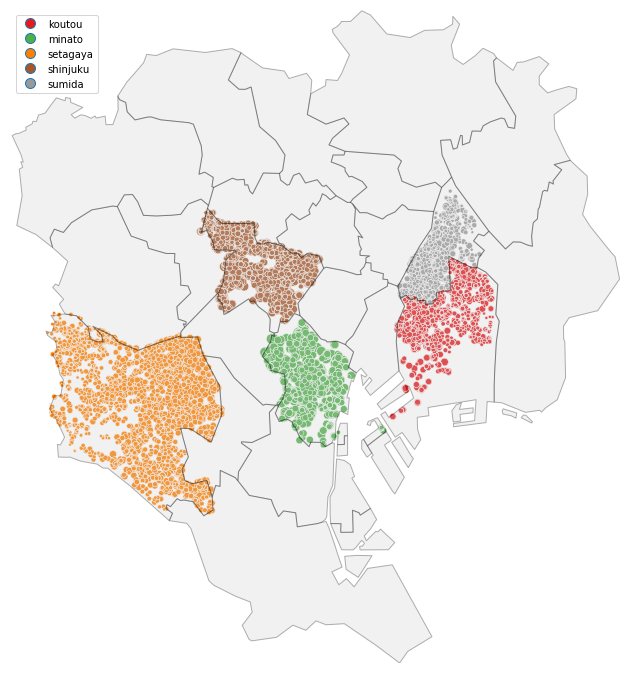
\includegraphics[scale=0.75]{sampledata.png}
\caption{Geographic Plot of Sample Data.\\
\textit{Notes}: The figure shows the geographic plot of sample data in our final dataset. Each point represents the geographic location of one observation. The size of each point represents the relative value (higher value, larger size) of rent per square meter of this observation. Different color represents different district.}
\label{fig1}
\end{figure}

\begin{figure}
\centering
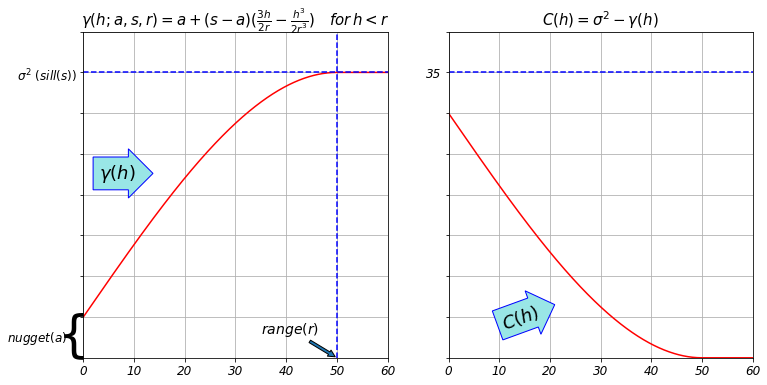
\includegraphics[scale=0.5]{variogram.png}
\caption{Theoretical Semi-Variogram (Left) and Co-Variogram (Right) for spherical model. \\
\textit{Notes}: The figure shows the theoretical Semi-Variogram function and Co-Variogram function with parameters nugget (a) equals to 5, sill (s) equals to 35, and range (r) equals to 50. }
\label{fig2}
\end{figure}

\begin{figure}
\centering
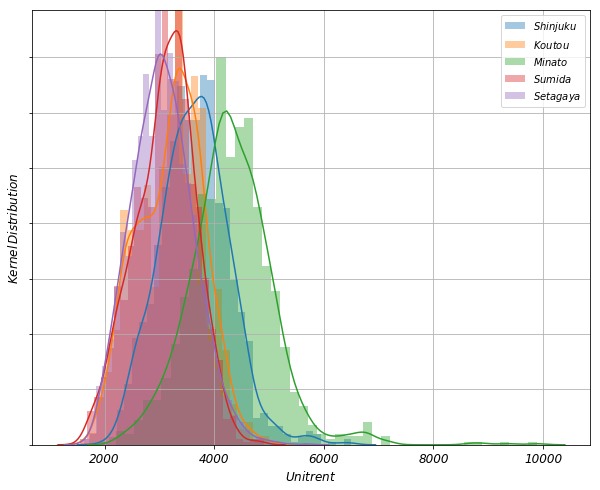
\includegraphics[scale=0.7]{kerneldist.png}
\caption{Kernel Distributions of rent per square meter, \var{Unitrent}, for five districts. \\
\textit{Notes}: The figure shows Kernel Distributions of rent per square meter for five districts. X-axis indicates the Kernel Distribution Probability and y-axis indicates the rent per square meter. Different color represents different district.}
\label{fig3}
\end{figure}

\newpage
\begin{landscape}
\begin{figure}
\centering
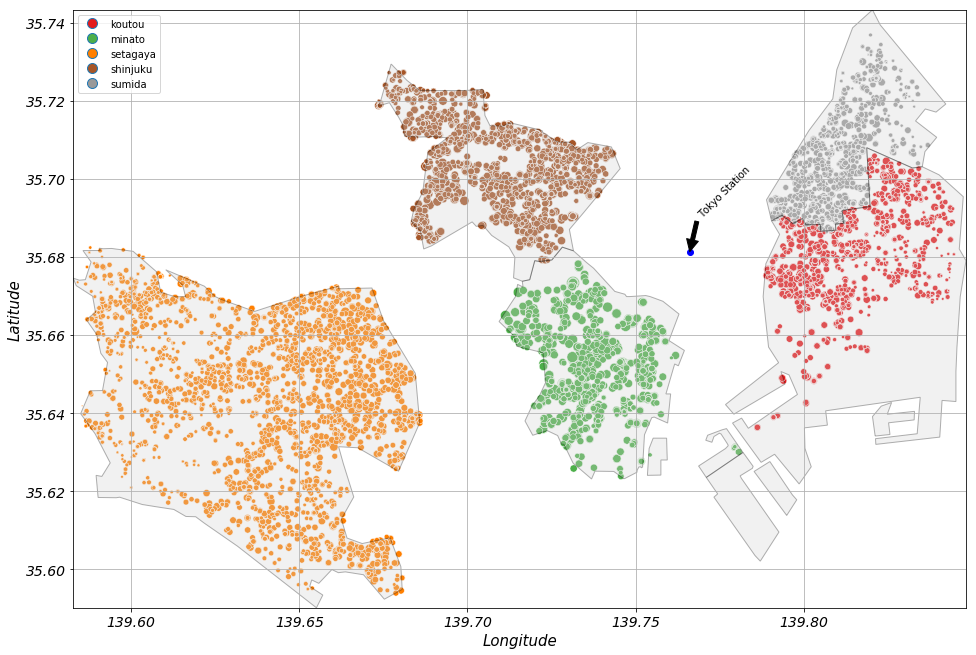
\includegraphics[scale=0.5]{interpretation.png}
\caption{Geographic interpretation of baseline regression results. \\
\textit{Notes}: The figure shows the relative position between each district and Tokyo Station. The size of the circle indicates the relative value of rent per square meter (larger circle larger \var{Unitrent}).}
\label{fig4}
\end{figure}
\end{landscape}

\newpage
\begin{figure}
\label{fig5}
\def\tabularxcolumn#1{m{#1}}
\begin{tabularx}{\linewidth}{@{}cXX@{}}
%
\begin{tabular}{cc}
\subfloat[a. Shinjuku District]{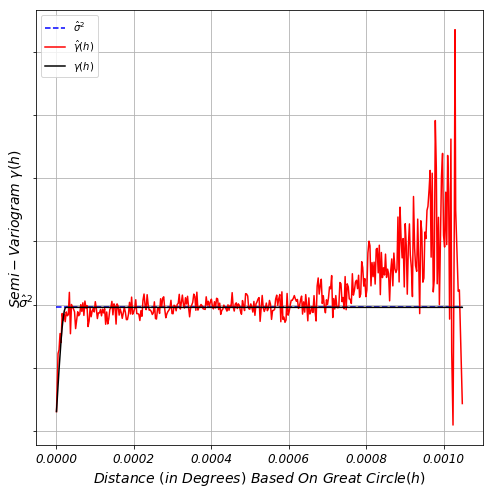
\includegraphics[scale=0.4]{shinjuku.png}} 
   & \subfloat[b. Koutou District]{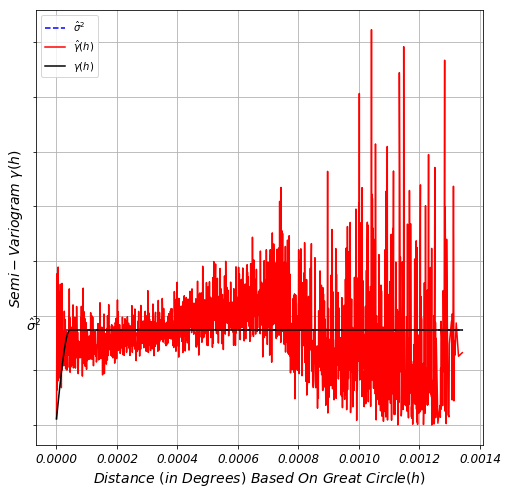
\includegraphics[scale=0.4]{koutou.png}}\\
\subfloat[c. Minato District]{\includegraphics[scale=0.4]{Minato.png}} 
   & \subfloat[d. Sumida District]{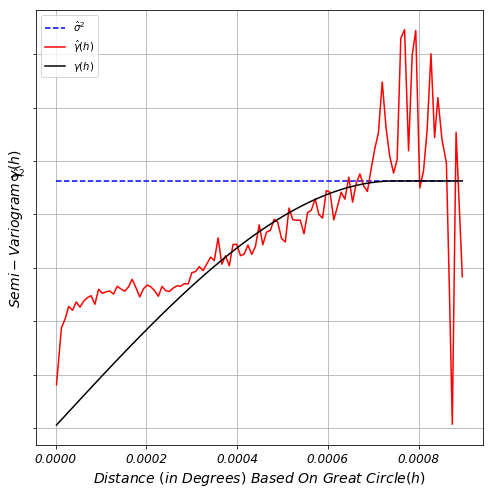
\includegraphics[scale=0.4]{sumida.png}}\\
\subfloat[e. Setagaya District]{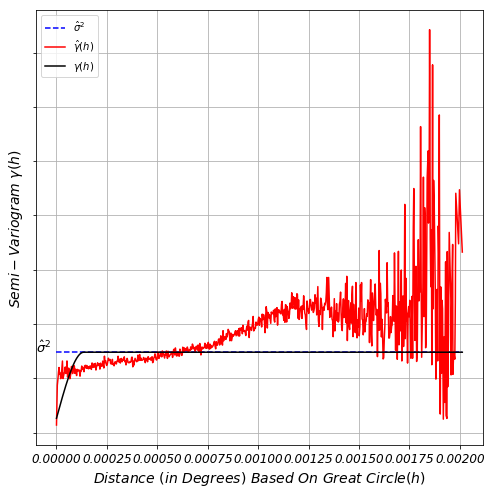
\includegraphics[scale=0.4]{setagaya.png}} 
   & \\
\end{tabular}
\end{tabularx}
\caption{Empirical Semi-Variograms for five districts. \\
\textit{Notes}: The red line represents actual binned semi-variogram, the black line represents fitted theoretical semi-variogram and the dashed blue line represents sill.}
\end{figure}

\newpage
\begin{landscape}
\begin{figure}
\centering
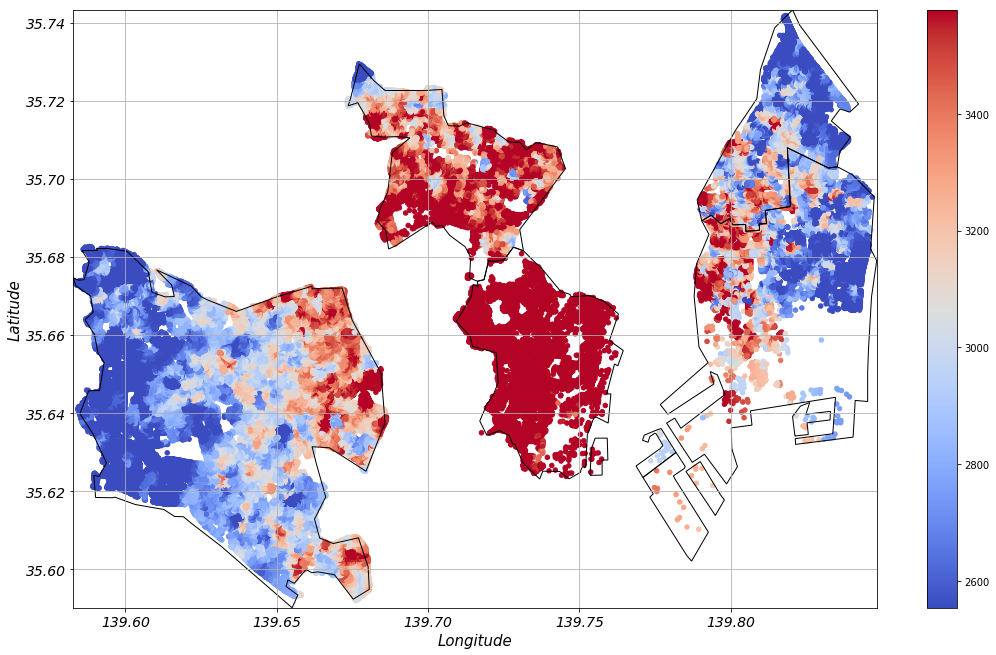
\includegraphics[scale=0.5]{ols.png}
\caption{Automated Valuation Model (AVM) based on OLS for five districts in Tokyo. \\
\textit{Notes}: The figure shows geographic plot of our Automated Valuation Model based on OLS method. All the residential buildings in our “point” dataset are plotted as color dots on this figure. The red-blue heatmap captures the relative value of rent per square meter for each dot. The value-range of heat map is located at the right of the map. X-axis and y-axis represents longitude and latitude respectively. 
} 
\label{fig6}
\end{figure}
\end{landscape}

\newpage
\begin{landscape}
\begin{figure}
\centering
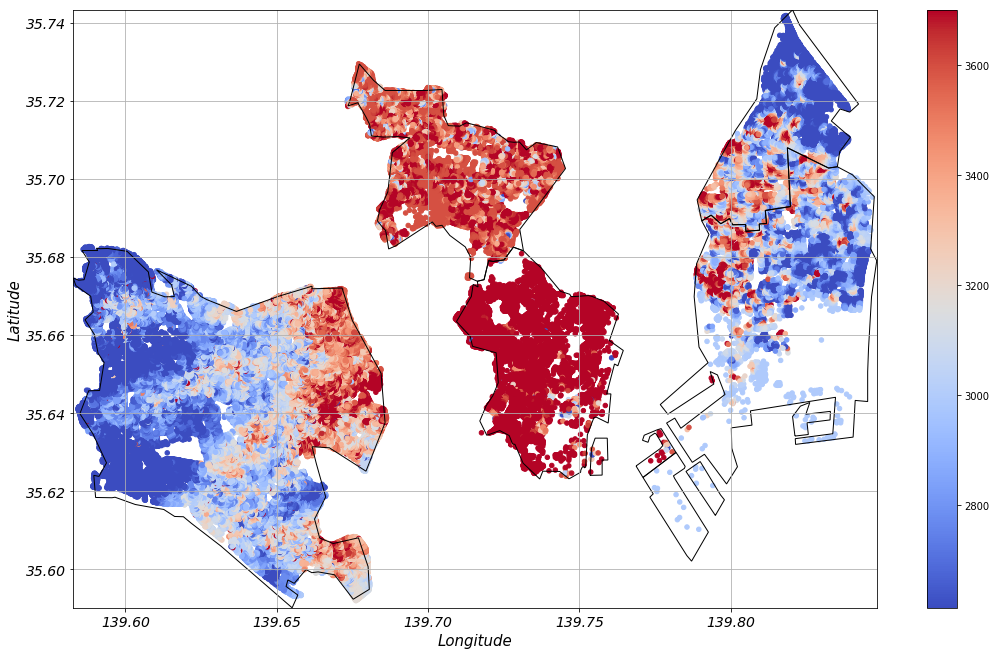
\includegraphics[scale=0.5]{kriging.png}
\caption{Automated Valuation Model (AVM) based on Ordinary Kriging for five districts in Tokyo. \\
\textit{Notes}: The figure shows geographic plot of our Automated Valuation Model based on Orinary Kriging method. All the residential buildings in our “point” dataset are plotted as color dots on this figure. The red-blue heatmap captures the relative value of rent per square meter for each dot. The value-range of heat map is located at the right of the map. X-axis and y-axis represents longitude and latitude respectively. 
} 
\label{fig7}
\end{figure}
\end{landscape}

\newpage
\begin{landscape}
\begin{figure}
\centering
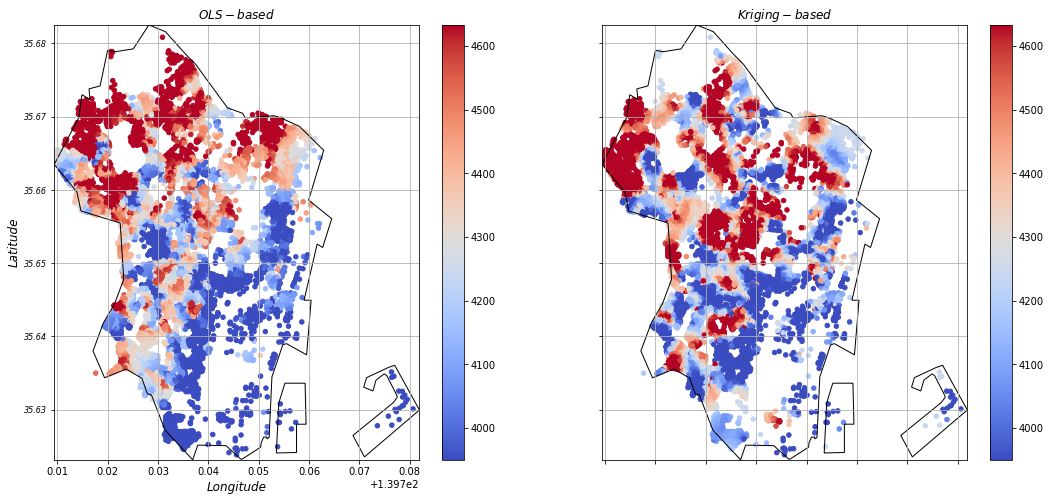
\includegraphics[scale=0.5]{minato_compare.png}
\caption{Automated Valuation Model for Minato districts based on OLS (Left) and Ordinary Kriging (Right). \\
\textit{Notes}: The figure shows geographic plot of our Automated Valuation Model based on OLS (Left) and Ordinary Kriging (Right). All the residential buildings in our “point” dataset are plotted as color dots on this figure. The red-blue heatmap captures the relative value of rent per square meter for each dot. The value-range of heat map is located at the right of the map. X-axis and y-axis represents longitude and latitude respectively. }
\label{fig8}
\end{figure}
\end{landscape}




\clearpage
\bibliographystyle{plainnat}
\bibliography{ref}
\end{document}
